\documentclass[12pt]{article}

% ── Packages ──────────────────────────────────────────────────────────────────
\usepackage[margin=1in]{geometry}
\usepackage{graphicx}
\graphicspath{{Figures/}}
\usepackage[font=small,labelfont=bf]{caption}

% Better Times New Roman font
\usepackage{newtxtext,newtxmath}

\usepackage{microtype}
\usepackage{setspace}
\usepackage{titlesec}
\usepackage{parskip}
\usepackage{ragged2e}   % Needed for \justifying
\usepackage{hyperref}
\usepackage{enumitem}
\usepackage{amsmath}
\usepackage{booktabs}
\usepackage[numbers,sort&compress]{natbib}
\usepackage{float}

% ── Page & Typography Setup ───────────────────────────────────────────────────
\singlespacing

\setlength{\parindent}{1.5em}
% \setlength{\parskip}{4pt}

\justifying   % Fully justified text

% ── Section Numbering & Formatting ───────────────────────────────────────────
\titleformat{\section}{\normalfont\large\bfseries}{\thesection}{0.75em}{}
\titleformat{\subsection}{\normalfont\normalsize\bfseries}{\thesubsection}{0.65em}{}
\titleformat{\subsubsection}{\normalfont\normalsize\itshape}{\thesubsubsection}{0.55em}{}

\titlespacing{\section}{0pt}{14pt}{4pt}
\titlespacing{\subsection}{0pt}{10pt}{2pt}
\titlespacing{\subsubsection}{0pt}{8pt}{2pt}

% ── Metadata ─────────────────────────────────────────────────────────────────
\title{%
  \textbf{Graph Neural Networks for Multi-Domain Routing Optimization}\\[6pt]
  \large Term Paper
}

\author{}  % We will manually format authors on title page
\date{}

% ══════════════════════════════════════════════════════════════════════════════
\begin{document}
% ══════════════════════════════════════════════════════════════════════════════

\begin{titlepage}
\centering

\vspace*{1cm}


\includegraphics[width=0.18\textwidth]{iitkgp_logo}\\[0.8cm]

{\Large \textbf{Graph Neural Networks for Multi-Domain Routing Optimization}}\\[10pt]
{\large Term Paper}\\[1.5cm]

\textbf{Submitted by:}\\[6pt]
\textbf{Group 3} \\
Datta Ksheeraj\\
Paramananda Bhaskar\\
Deetosh Kumar Kuila\\ [0.5cm]
\textbf{Group 11} \\
Krishna Singha \\
Sukumar Singh \\
Harsh Chattar \\[1.2cm]

\textbf{Course:} Internet Architecture and Protocols\\
\textbf{Instructor:} Prof.\ Soumya Kanti Ghosh\\[1.2cm]

\textbf{Department of Computer Science and Engineering}\\
Indian Institute of Technology Kharagpur\\[1.5cm]

\textbf{Date:} \today

\vfill

\end{titlepage}

\newpage
\section*{Author Contributions}
We state here the primary contributor of each section in this paper. 
\begin{itemize}
    \item \textbf{Datta Ksheeraj}: Topology generation pipeline (random, scale-free, mesh, ring, hybrid graphs), multi-domain AS-like partitioning, and node/edge attribute assignment.
    \item \textbf{Paramananda Bhaskar}: Ground-truth latency labelling using M/M/1 and M/G/1 queueing models, bottleneck identification, and export pipeline (JSON, GraphML, CSV formats).
    \item \textbf{Deetosh Kumar Kuila}: Traffic simulation --- diurnal load variation, flash-crowd events, application-profile demand matrices, and temporal snapshot generation.
    \item \textbf{Krishna Singha}: Feature engineering (node, edge, and global feature arrays), dataset assembly into PyTorch Geometric format, and RouteNet-Fermi dataset augmentation with path--link COO tensors.
    \item \textbf{Sukumar Singh}: GNN model implementation (GCN, GAT, MPNN, EdgeWeightGNN, SpatialTemporalGNN), training loop with per-model peak configurations and early stopping, and checkpoint management.
    \item \textbf{Harsh Chattar}: RouteNet-Fermi implementation and architectural fixes (normalised-sum aggregation, demand path features), comprehensive benchmark pipeline, statistical evaluation, and report writing.
\end{itemize}

\thispagestyle{empty}
\newpage

\thispagestyle{empty}
\newpage

\tableofcontents
\newpage

% ══════════════════════════════════════════════════════════════════════════════
\section{Abstract}
Graph Neural Networks (GNNs) are increasingly promising for network performance modeling, but their effectiveness depends heavily on the quality of the data used for training and evaluation. This paper focuses on the dataset generation, network modeling, GNN model development, congestion-aware routing optimization, and evaluation layers of a larger multi-domain routing optimization project. 

We design a synthetic yet realistic pipeline that generates 500+ Internet-like topologies, partitions them into AS-like domains, and annotates them with node, edge, and global features that capture structural and traffic-related network state. The resulting dataset is exported in interoperable formats and is intended to serve as a shared foundation for downstream learning-based routing experiments. Traffic matrices are a central abstraction in network engineering, and both topology and traffic structure must be represented carefully to support meaningful prediction and optimization tasks \cite{internetTrafficMatrices}. To make the dataset useful for congestion-aware routing research, we also simulate time-varying traffic with diurnal variation, flash-crowd events, and application-dependent demand patterns, and we derive ground-truth latency labels using queueing-based models \cite{internetTrafficMatrices,mm1}. This design follows the broader direction of recent network modeling work, where topology, routing, and traffic are treated jointly rather than independently. 

Building on this dataset, the paper further presents GNN model development for predicting network performance, a congestion-aware routing optimizer that selects paths based on predicted latency instead of traditional metrics, and an evaluation comparing the proposed approach with baseline routing strategies under varying network conditions. 

% ══════════════════════════════════════════════════════════════════════════════
\section{Introduction}
Modern networks carry traffic that changes over time, crosses multiple domains, and often faces congestion in unexpected places. In such settings, routing decisions cannot rely only on simple static rules such as hop count, because the best path depends on the current network state, link capacity, and traffic load. At the same time, Graph Neural Networks (GNNs) have become a strong option for network performance modeling because they are designed to work on graph-structured data and can learn relationships between topology, routing, and traffic. RouteNet is a well-known example of this direction, showing that a GNN can be used to predict key performance metrics by modeling these network relationships jointly \cite{routeNet}.

A major challenge in this area is that good learning-based routing models require good data. Real network measurements are often hard to obtain, incomplete, or not suitable for controlled experiments, so synthetic network generation is still widely used in networking research. BRITE \cite{brite} was developed as a universal topology generation tool for this purpose, and later work such as Inet focused on Internet-like topology generation at the AS level. In parallel, traffic matrices have long been recognized as a central abstraction in network engineering, since they summarize the demand between source and destination pairs and are widely used in traffic engineering and planning \cite{internetTrafficMatrices}.

This paper addresses both needs together. On the data side, we generate a large set of synthetic Internet-like topologies, divide them into AS-like domains, and attach node, edge, and global features that describe the network structure and its traffic-related state. We also generate time-varying traffic patterns with diurnal changes, flash-crowd events, and application-dependent demand, and we compute latency labels using queueing-based models so that the dataset reflects congestion effects rather than only static connectivity. Queueing delay and realistic traffic synthesis have both been studied in prior network research, which supports the use of these methods for creating meaningful ground truth \cite{internetTrafficMatrices}.

On the modeling side, the paper builds GNN-based predictors that learn from these graph representations and estimate network performance under different load conditions. These predictions are then used in a congestion-aware routing optimizer that selects paths based on predicted latency instead of fixed metrics alone. The final part of the paper evaluates the full system against baseline routing strategies and compares how well the learned approach handles changing traffic and congestion. In this way, the paper presents a complete pipeline that combines dataset generation, network modeling, GNN development, routing optimization, and evaluation for multi-domain routing research.

% ══════════════════════════════════════════════════════════════════════════════
\section{Related Work}
\label{sec:related_work}
% ══════════════════════════════════════════════════════════════════════════════

\subsection{Graph Neural Networks}
Graph Neural Networks (GNNs) extend deep learning to irregularly structured graph data by iteratively aggregating information from node neighbourhoods. Kipf and Welling introduced Graph Convolutional Networks (GCN) \cite{gcnKipf}, which apply a spectral-motivated aggregation rule that weights all neighbours equally via the symmetric normalized adjacency matrix. Veličković et al.\ proposed Graph Attention Networks (GAT) \cite{gatVelickovic}, replacing the fixed weights with learned attention coefficients, allowing the model to prioritize more informative neighbours. Gilmer et al.\ formulated a general Message Passing Neural Network (MPNN) framework \cite{mpnnGilmer} in which edge-conditioned linear transformations (NNConv) map each edge's feature vector to a per-edge weight matrix, letting edge properties modulate the messages flowing along each link. These three architectures span a spectrum from simple uniform aggregation to fully edge-conditioned propagation, and they form the foundational baselines evaluated in this paper.

For temporal modelling, Vaswani et al.\ \cite{transformerVaswani} introduced the Transformer architecture, which replaces recurrence with self-attention over a sequence. Self-attention can attend directly to any past step without vanishing-gradient degradation, making it well-suited for learning long-range dependencies in traffic time series.

\subsection{GNN-Based Network Performance Modeling}
RouteNet \cite{routeNet} demonstrated that GNNs can accurately predict key Quality-of-Service (QoS) metrics in packet networks by jointly modeling topology, routing, and traffic. Its successor, RouteNet-Fermi, extended this to a heterogeneous bipartite graph that maintains separate hidden states for network links and source-destination paths. By alternately propagating information from paths to links and from links back to paths through GRU-gated scatter operations, RouteNet-Fermi can capture the shared-resource congestion effects that a standard node-only GNN cannot represent. These papers establish a strong case for domain-specific architectural inductive biases when modeling network performance, motivating this work's inclusion of RouteNet-Fermi alongside general-purpose GNNs.

\subsection{Synthetic Network Topology Generation}
Synthetic topology generation has a long history in networking research. Medina et al.\ developed BRITE \cite{brite} as a universal topology generator supporting multiple models including Barabási-Albert and Waxman, arguing that a good generator must be representative, flexible, and composable. Barabási and Albert showed that many real-world networks, including the Internet's AS-level graph, exhibit scale-free degree distributions arising from preferential attachment \cite{barabasiAlbert}. This motivates the inclusion of scale-free topologies in the dataset generated for this work alongside random, mesh, ring, and hybrid structures, ensuring that the training data spans a realistic diversity of connectivity patterns.

\subsection{Traffic Matrices and Queueing Models}
Traffic matrices are a central abstraction in network engineering, summarizing the aggregate demand between all source-destination pairs. Zhang et al.\ \cite{internetTrafficMatrices} developed efficient methods for estimating large-scale IP traffic matrices from link-load measurements, highlighting the engineering importance of these structures. Nucci et al.\ \cite{itmgen} studied the problem of generating synthetic traffic matrices that accurately reflect real interdomain traffic, noting that application type, AS size, and regional demand must all be modeled. Leland et al.\ showed that Ethernet traffic is self-similar and bursty, not smooth and Poisson-like, making log-normal demand and diurnal variation appropriate choices for synthetic traffic generation \cite{ethernetTraffic}. Queueing models provide the analytical bridge from traffic demand to link delay: the M/M/1 model \cite{mm1} and its extensions \cite{queueDelay} are standard tools for computing expected latency under varying utilization, and they are used in this work to generate ground-truth labels for all static load conditions.

% ══════════════════════════════════════════════════════════════════════════════
\section{Dataset Creation and Network Modeling}
\label{sec:features}
% ══════════════════════════════════════════════════════════════════════════════

\subsection{Overview}
This part of the project builds the data foundation for the whole routing system. The reason for doing this is simple: graph learning methods require graph-structured data that is realistic enough to represent network behavior, while still being controlled enough to support repeatable and scalable experiments. Since real-world network datasets are often incomplete, inaccessible, or unsuitable for controlled evaluation, synthetic data generation is commonly used to create diverse and well-structured network scenarios. The goal here is to generate a dataset that captures important characteristics of real networks, such as topology diversity, multi-domain structure, and dynamic traffic behavior, while maintaining consistency and reproducibility across all generated instances.

\subsection{Dataset Configuration and Scale}
In this implementation, the dataset is designed to generate a total of 500 network topologies with a balanced mix of different graph types, including random, scale-free, mesh, ring, and hybrid structures. The size of each topology varies between 10 and 100 nodes, and every network is divided into 2 to 5 domains to reflect a multi-domain setting. Along with topology generation, the pipeline defines four fixed load levels for computing static latency labels and simulates 12 time steps per topology to capture changes in traffic over time. It also allows the use of different queueing models (M/M/1 or M/G/1) \cite{mm1}, includes random flash-crowd events, and limits the number of paths sampled in each snapshot to keep the data manageable. Overall, these design choices ensure that the dataset is diverse and realistic, while still being computationally efficient to generate and analyze.

\subsection{Topology Generation}
The topology generator is implemented with NetworkX \cite{networkX} and produces several different graph families: random graphs, scale-free graphs, mesh graphs, ring graphs, and hybrid small-world graphs. Each family covers a different network shape. Random graphs create irregular connectivity, scale-free graphs capture hub-heavy structures, mesh graphs resemble regular backbone layouts, ring graphs provide resilient cyclic structure, and hybrid graphs mix local clustering with long-range shortcuts. This diversity matters because the downstream learning model should not only see one type of graph. BRITE explicitly argues that a good topology generator should be representative, flexible, and able to combine multiple generation models \cite{brite}; that is exactly the motivation behind using several topology families instead of a single synthetic pattern.

\subsection{Multi-Domain Structure}
A multi-domain, AS-like structure is incorporated into each generated topology to better reflect real-world network organization. Nodes are partitioned into multiple domains, and each domain is assigned a spatial center so that node coordinates form clustered regions rather than random distributions. This results in topologies that more closely resemble inter-domain Internet structures instead of simple undirected graphs. In addition, inter-domain links are introduced as a sparse backbone connecting different domains, while the majority of links remain within individual domains. This distinction is important because routing in real networks is influenced by administrative boundaries, peering relationships, and policy constraints, rather than relying solely on shortest-path distance. Interdomain traffic studies such as ITMgen further support this approach by treating the AS level as a suitable abstraction for modeling interdomain connectivity and traffic behavior \cite{itmgen}.

\subsection{Node Feature Representation}
Each node in the generated topology is annotated with a set of features that capture both its structural role and its expected behavior within the network. These features are chosen to provide meaningful input signals for graph-based learning models, as prior work has shown that combining topology with node and link attributes improves the accuracy of network performance prediction. In particular, approaches such as RouteNet highlight that network behavior cannot be inferred from connectivity alone, but requires additional contextual information about nodes and traffic \cite{routeNet}.

The following node attributes are included in our implementation:
\begin{itemize}
    \item \textbf{Router type (core, edge, gateway)}: This attribute represents the functional role of the router within the network. Core routers typically handle high-volume transit traffic, edge routers connect end hosts, and gateway routers manage inter-domain communication. Including router type allows the model to distinguish between nodes with different responsibilities, which is important because traffic patterns and load characteristics vary across these roles.
    \item \textbf{Capacity (in Mbps)}: This defines the processing or forwarding capability of the router. Nodes with higher capacity can handle more traffic without congestion, while low-capacity nodes are more likely to become bottlenecks. This attribute is essential for modeling realistic network behavior, as capacity constraints directly influence routing performance and latency.
    \item \textbf{Spatial coordinates (x, y)}: Each node is assigned a position in a 2D space to approximate its physical or geographical location. These coordinates are used to compute propagation delay between nodes and to create clustered domain structures. This reflects the fact that latency in real networks is partly determined by physical distance.
    \item \textbf{Domain ID}: This attribute identifies the domain (or AS-like group) to which the node belongs. It enables the model to distinguish between intra-domain and inter-domain communication, which is important because routing policies and link characteristics often differ across domain boundaries.
    \item \textbf{Historical traffic (baseline load factor)}: This represents the typical traffic load associated with the node. It is later used to scale traffic generation, ensuring that some nodes consistently generate or receive more traffic than others. This helps simulate realistic traffic distributions where demand is uneven across the network.
\end{itemize}

These attributes are selected to ensure that the dataset captures both structural and operational aspects of the network. By providing information about node roles, capacity limits, spatial placement, and traffic tendencies, the dataset enables learning models to better understand how congestion forms and propagates.

\subsection{Edge Feature Representation}
Each edge in the generated topology is annotated with a set of attributes that capture the physical, structural, and operational properties of network links. These features are essential because, in real networks, link-level characteristics such as capacity, delay, and reliability directly influence congestion, routing decisions, and overall performance. Prior work in network modeling, particularly RouteNet and its extensions \cite{routeNet}, shows that link attributes such as capacity and delay must be explicitly modeled, as performance metrics like latency and packet loss depend on both topology and link-specific properties rather than connectivity alone.

The following edge attributes are included in our implementation:
\begin{itemize}
    \item \textbf{Bandwidth (in Mbps)}: This represents the maximum transmission capacity of the link. It is one of the most important factors in determining congestion, as links with lower bandwidth are more likely to become bottlenecks under high traffic. Assigning different bandwidth ranges to intra-domain and inter-domain links reflects real-world networks, where backbone or inter-domain links often have different provisioning compared to local links.
    \item \textbf{Propagation Delay (in ms)}: This captures the time required for a signal to travel across the link. It is computed based on the geometric distance between nodes, with added noise to avoid uniformity. This reflects the fact that latency in real networks is partly determined by physical distance. Traffic engineering literature commonly models delay as a combination of propagation delay and queueing delay, making this attribute essential for realistic latency estimation.
    \item \textbf{Inter-domain Flag}: This indicates whether a link connects nodes from different domains (AS-like structures). This attribute is important because inter-domain links often have different performance characteristics and are subject to policy constraints. Interdomain routing studies, such as ITMgen, treat the AS level as a key abstraction, showing that traffic patterns and connectivity differ significantly across domain boundaries \cite{itmgen}.
    \item \textbf{Link Reliability}: This represents the stability or failure probability of the link. While not always explicitly modeled in basic topology generators, reliability is an important practical consideration in network design and routing, as unreliable links can degrade performance and increase packet loss. Including this attribute allows the dataset to capture variability in link quality and supports more robust routing decisions.
    \item \textbf{Cost}: This is a composite metric derived from propagation delay and a penalty based on bandwidth. It reflects the trade-off between latency and capacity, which is central to traffic engineering. Instead of using hop count alone, modern routing approaches consider multiple factors, including delay and congestion risk. Traffic engineering literature emphasizes that optimal routing decisions should balance these factors rather than relying solely on shortest paths \cite{internetTrafficMatrices}.
\end{itemize}

Overall, these edge features ensure that the dataset captures both the physical characteristics and operational constraints of network links. By combining capacity, delay, domain structure, and reliability, the dataset provides a richer representation of the network, enabling learning models to better understand how congestion forms and how routing decisions impact performance.

\subsection{Traffic Modeling}
Traffic is generated as a time-varying source–destination matrix rather than as a single static demand table. This is important because the network does not carry the same load at all times, and a realistic dataset must reflect changes over time, different application types, and uneven demand across domains. The traffic-matrix literature treats temporal variation, spatial variation, and spatio-temporal variation as separate modeling concerns, while ITMgen shows that simple gravity-style traffic models are not enough because application type, AS size, and regional popularity all affect interdomain traffic \cite{itmgen}. The same general idea is also supported by classic traffic studies showing that Internet traffic is bursty and self-similar rather than smooth and Poisson-like \cite{ethernetTraffic}.

For each topology with $N$ nodes, the simulator builds a traffic matrix 
$M_t \in \mathbb{R}^{N \times N}$ at timestep $t$, where each entry 
$M_t[i,j]$ represents the traffic demand (in Mbps) from source node $i$ 
to destination node $j$. Self-traffic is excluded, so 
$M_t[i,i] = 0$ for all $i$.

The matrix is not generated uniformly. Instead, each demand value is 
influenced by multiple factors, including diurnal variations, 
flash-crowd events, application-specific behavior, and domain-level 
structure. This results in more realistic traffic patterns and makes 
the generated dataset suitable for congestion-aware routing experiments.

\subsubsection{Temporal load variation}
The first factor is the diurnal multiplier, which models how traffic changes over a simulated day. The code uses a sinusoidal function:
\[
d(t) = 0.70 + 0.45 \cdot \frac{1 + \sin\left(\frac{2\pi t}{T} - \frac{\pi}{2}\right)}{2},
\]
where $T$ is the total number of timesteps. This results in values in the range $[0.70, 1.15]$, so traffic is lower at one part of the cycle and higher at another. This is a simple but effective way to represent the fact that network load changes over time rather than remaining constant.

\subsubsection{Flash-crowd events}
The second factor is the flash-crowd multiplier. At each timestep, the simulator draws a random event with probability $p_f$. If a flash crowd occurs, traffic is multiplied by a random factor:
\[
f(t) \sim U(1.8, 3.4).
\]
Otherwise,
\[
f(t) = 1.
\]
This creates sudden spikes in load, which are useful for testing whether the GNN can handle congestion under abrupt demand changes. Such bursty behavior is consistent with classic Internet traffic studies, which shows traffic is not smooth and can exhibit bursts across many time scales \cite{ethernetTraffic}.

\subsubsection{Application profiles}
The simulator also samples one of three application profiles:
\begin{itemize}
    \item \textbf{web} with probability $0.55$
    \item \textbf{video} with probability $0.25$
    \item \textbf{bulk} with probability $0.20$
\end{itemize}

Each profile has its own scale and variance parameters:
\begin{itemize}
    \item \textbf{web}: mean scale $0.5$, $\sigma = 0.6$
    \item \textbf{video}: mean scale $1.1$, $\sigma = 0.4$
    \item \textbf{bulk}: mean scale $0.9$, $\sigma = 1.0$
\end{itemize}

This is done because different traffic classes have different shapes. Web traffic is usually lighter and more bursty, video traffic is heavier but steadier, and bulk transfers often produce large flows with more variation. ITMgen supports this kind of modeling explicitly by arguing that application type and content popularity must be included when generating interdomain traffic matrices \cite{itmgen}.

\subsubsection{Log-normal base demand}
For each source--destination pair $(i,j)$, the base demand is sampled from a log-normal distribution:
\[
X_{ij} \sim \text{LogNormal}(\mu = 0.1,\ \sigma = \sigma_a)
\]

where $\sigma_a$ depends on the selected application profile. A log-normal distribution is a good choice here because it naturally produces many small values and a few large values, which matches the uneven structure of real network traffic. This is especially useful when generating heterogeneous source--destination demand, because real traffic often has a long tail rather than a narrow symmetric shape.


\subsubsection{Final demand formula}

The final traffic demand used in the matrix is computed as:
\[
D_{ij}(t) = X_{ij} \cdot s_a \cdot d(t) \cdot f(t) \cdot b_{ij} \cdot (0.5 + h_i)
\]

where:
\begin{itemize}
    \item $X_{ij}$ = log-normal base demand
    \item $s_a$ = application mean scale
    \item $d(t)$ = diurnal factor
    \item $f(t)$ = flash-crowd multiplier
    \item $b_{ij}$ = inter-domain boost
    \item $h_i$ = historical traffic of source node $i$
\end{itemize}

The inter-domain boost is defined as:
\[
b_{ij} =
\begin{cases}
1.3, & \text{if } \mathrm{domain}(i) \neq \mathrm{domain}(j) \\
1.0, & \text{otherwise}
\end{cases}
\]

This gives slightly higher demand to cross-domain flows, which is reasonable in an AS-like setting because interdomain traffic is often more aggregated and more policy-sensitive than purely local traffic. The historical traffic factor $(0.5 + h_i)$ scales outgoing demand so that some routers consistently generate more traffic than others. This helps the dataset reflect uneven load distribution instead of making all nodes behave the same way.

\subsubsection{Global metadata}
For each timestep, the simulator also stores a small set of global features: time of day, diurnal factor, flash event, flash multiplier, traffic profile, and network load in Mbps.

These values are important because they summarize the network condition at the snapshot level and can later be used by the GNN as global context. The total network load is simply:
\[
L_t = \sum_{i \neq j} D_{ij}(t)
\]

which is stored as network load. This makes every snapshot self-contained: it includes the traffic matrix, the global traffic condition, and the labels that will later be used for performance prediction.

\subsection{Ground-Truth Latency Generation}
Ground-truth latency labels are generated at two levels: static (load-controlled) and temporal (traffic-driven). This two-level design is important because it provides both clean baseline labels under fixed conditions and realistic labels under dynamic traffic. In network modeling, latency is typically decomposed into propagation delay and queueing delay, where queueing delay depends on link utilization and traffic variability. This approach is widely used in both queueing theory and network performance modeling literature \cite{queueDelay}.

\subsubsection{Static Latency Modeling (Fixed Load Conditions)}

In the static setting, latency is computed for a set of predefined utilization levels:
\[
\rho \in \{0.20, 0.50, 0.80, 0.95\},
\]
corresponding to low, medium, high, and near-congested (flash) conditions.

For each edge, the service rate is derived from its bandwidth and the average packet size:
\[
\mu = \frac{C}{S},
\]
where $C$ is the link bandwidth (in Mbps) and $S = 0.001$ Mb is the average packet size. The arrival rate is then:
\[
\lambda = \rho \cdot \mu.
\]

Using an M/M/1 queueing model, the average queueing delay is:
\[
W_q = \frac{\rho}{\mu (1 - \rho)}.
\]

The total latency on an edge is computed as:
\[
L = d_{\text{prop}} + W_q,
\]
where $d_{\text{prop}}$ is the propagation delay derived from node distance.

This formulation ensures that latency increases rapidly as utilization approaches 1, capturing the nonlinear behavior of congestion. The use of M/M/1 is common in networking because it provides a simple analytical approximation of delay under stochastic arrivals, even though real traffic may deviate from exponential assumptions.

\subsubsection{Temporal Latency Modeling (Traffic-Driven Simulation)}
In the temporal setting, latency is derived from the simulated traffic matrix at each timestep. The process follows three main steps:
\begin{itemize}
    \item \textbf{Traffic Routing and Load Accumulation}: 
    For each source--destination pair $(i,j)$, the demand $D_{ij}(t)$ is routed through the network using a weighted shortest-path algorithm. The edge weight is defined as
    \[
    w_e = d_{\mathrm{prop}} + \alpha \cdot \frac{1}{C},
    \]
    where $C$ is the link bandwidth and $\alpha$ is a scaling factor. This formulation penalizes low-capacity links, encouraging traffic to flow through higher-capacity paths. This is consistent with traffic engineering principles, where routing decisions aim to balance delay and congestion rather than minimize hop count alone.
    
    As traffic is routed, the load on each edge is accumulated as
    \[
    L_e(t) = \sum_{(i,j)\in P_e} D_{ij}(t),
    \]
    where $P_e$ is the set of source--destination pairs whose paths include edge $e$.

    \item \textbf{Utilization and Queueing Metrics}
    For each edge, utilization is computed as
    \[
    \rho_e(t) = \frac{L_e(t)}{C_e}.
    \]
    
    Based on this utilization, queueing delay is calculated using either:
    
    \[
    W_q = \frac{\rho}{\mu (1 - \rho)}.
    \]

    \[
    W_q = \frac{\lambda \cdot \mathbb{E}[S^2]}{2(1 - \rho)},
    \]
    where $\mathbb{E}[S^2]$ is the second moment of the service time. The M/G/1 model is included because real network traffic is often bursty and does not follow exponential service distributions. This aligns with studies showing that Internet traffic exhibits heavy-tailed and self-similar behavior.
    
    Queue length is also estimated as
    \[
    Q = \lambda \cdot W_q,
    \]
    which provides an additional indicator of congestion buildup.

    \item \textbf{Latency and Bottleneck Identification}
    The total latency for each edge is given by
    \[
    \ell_e(t) = d_{\mathrm{prop}} + W_q.
    \]
    
    Edges with utilization above a threshold (for example, the top percentile or $\rho > 0.9$) are marked as bottlenecks. This helps identify critical links where congestion is most severe.
    
    For each path, the end-to-end latency is computed as
    \[
    L_{\mathrm{path}} = \sum_{e \in P} \ell_e(t),
    \]
    and additional metrics such as hop count and bottleneck count are recorded.
        
\end{itemize}
This design is effective as it connects traffic demand $\rightarrow$ link load $\rightarrow$ queueing delay $\rightarrow$ latency, which represents the fundamental chain underlying congestion in packet networks. The static labels provide a stable baseline, while the temporal labels capture changing load and bottleneck formation over time. 

The weighted shortest-path step also makes the simulator more realistic for routing studies, as traffic-engineering literature shows that shortest-path routing can perform poorly when it ignores link capacity and congestion. The final dataset therefore provides the subsequent GNN model with both a meaningful learning target and a realistic congestion environment.

% ══════════════════════════════════════════════════════════════════════════════
\section{GNN Models for Latency Prediction}
\label{sec:models}
% ══════════════════════════════════════════════════════════════════════════════

\subsection{Task Formulation}
The learning task is formulated as a graph-level edge regression problem. Each sample in the dataset is a network topology represented as a directed graph $\mathcal{G} = (\mathcal{V}, \mathcal{E})$, where each node $v \in \mathcal{V}$ corresponds to a router and each directed edge $e \in \mathcal{E}$ corresponds to a unidirectional network link. The model must predict the steady-state end-to-end latency (in milliseconds) for each edge under a given traffic load condition. Four static load conditions (low, medium, high, and overload) are evaluated, providing a range from uncongested to heavily congested states. The per-edge latency arises from both the fixed propagation delay and the variable queueing delay induced by the traffic demand routed over each link.

\subsection{Shared Input Feature Schema}
All models receive the same three feature tensors constructed during preprocessing:

\begin{table}[h]
\centering
\caption{Node feature vector (12 dimensions per node)}
\begin{tabular}{lll}
\toprule
\textbf{Index} & \textbf{Feature} & \textbf{Description} \\
\midrule
0 & degree\_norm & Normalized node degree \\
1 & betweenness\_centrality & Betweenness centrality \\
2 & clustering\_coeff & Clustering coefficient \\
3 & avg\_link\_capacity & Mean outgoing link capacity \\
4 & avg\_neighbors\_degree & Mean degree of neighbors \\
5--6 & domain\_onehot & One-hot domain membership (2 dims) \\
7 & x\_coord & Normalized x-coordinate \\
8 & y\_coord & Normalized y-coordinate \\
9 & historical\_traffic & Normalized average traffic demand \\
10 & out\_degree\_norm & Normalized out-degree \\
11 & in\_degree\_norm & Normalized in-degree \\
\bottomrule
\end{tabular}
\end{table}

\begin{table}[h]
\centering
\caption{Edge feature vector (5 dimensions per edge)}
\begin{tabular}{lll}
\toprule
\textbf{Index} & \textbf{Feature} & \textbf{Description} \\
\midrule
0 & link\_capacity\_norm & Normalized link bandwidth capacity \\
1 & propagation\_delay\_norm & Normalized propagation delay \\
2 & current\_load & Fractional link utilization \\
3 & is\_cross\_domain & Binary inter-domain flag \\
4 & hop\_count\_norm & Normalized position in path \\
\bottomrule
\end{tabular}
\end{table}

\begin{table}[h]
\centering
\caption{Global feature vector (11 dimensions per graph)}
\begin{tabular}{lll}
\toprule
\textbf{Index} & \textbf{Feature} & \textbf{Description} \\
\midrule
0 & num\_nodes\_norm & Normalized node count \\
1 & num\_edges\_norm & Normalized edge count \\
2 & avg\_degree\_norm & Average node degree \\
3 & density & Graph edge density \\
4--8 & topology\_type\_onehot & One-hot type (5 dims: random, scale-free, mesh, ring, hybrid) \\
9 & avg\_capacity\_norm & Mean capacity across all links \\
10 & total\_demand\_norm & Total traffic demand in graph \\
\bottomrule
\end{tabular}
\end{table}

\subsection{Graph Convolutional Network (GCN)}
The GCN model \cite{gcnKipf} applies a symmetrically normalized message passing rule across two graph convolutional layers (hidden dimension 64), followed by a three-layer MLP edge decoder. For each edge $(u, v)$, the decoder concatenates the embeddings of the source node $h_u$, destination node $h_v$, and the edge feature vector $e_{uv}$, then predicts the latency through a ReLU-activated network. The GCN treats all neighbours equally (no edge weighting or attention), making it the simplest baseline. It has 16,484 trainable parameters and was trained with learning rate $5 \times 10^{-4}$, weight decay $10^{-5}$, for up to 200 epochs with early stopping (patience 25).

\subsection{Graph Attention Network (GAT)}
The GAT model \cite{gatVelickovic} replaces GCN's fixed symmetric weights with multi-head attention. Each of the two GAT layers uses 4 attention heads with hidden dimension 64, so the concatenated output per layer is 256-dimensional. The attention mechanism computes a scalar score for each neighbour as a function of the source and target node features, then softmax-normalizes the scores to produce weighted aggregation coefficients. This allows the model to focus on more informative neighbours within the local structure. The edge decoder mirrors the GCN architecture. GAT has 26,692 parameters and was trained with learning rate $5 \times 10^{-4}$, weight decay $10^{-5}$, for up to 200 epochs with early stopping (patience 25).

\subsection{Message Passing Neural Network (MPNN)}
The MPNN model \cite{mpnnGilmer} uses NNConv layers, in which a small neural network maps each edge's feature vector to a matrix that transforms the source-node embedding before aggregation. This makes the model fully edge-conditioned: the contribution of each neighbour is modulated by the properties (capacity, delay, load) of the connecting link. Two NNConv layers are applied (hidden dimension 64), followed by global mean pooling and the same MLP edge decoder. MPNN has the highest parameter count among the general-purpose baselines (308,068 parameters) due to the per-edge weight matrices. It was trained with learning rate $3 \times 10^{-4}$, weight decay $10^{-3}$, for up to 250 epochs with early stopping (patience 35).

\subsection{RouteNet-Fermi}
RouteNet-Fermi \cite{routeNet} is the key domain-specific model in this study. It represents the network as a heterogeneous bipartite graph with two node types — \emph{links} and \emph{paths} — and alternates message passing between them via GRU-gated aggregations. Each source-destination path is represented by its sequence of traversed links; the model iterates the following two steps: (1) \emph{Links$\leftarrow$Paths}: each link aggregates the hidden states of all paths that traverse it; (2) \emph{Paths$\leftarrow$Links}: each path updates its hidden state by aggregating the updated link states along its route.

\paragraph{Link aggregation.} To preserve the congestion signal — links shared by many paths should receive proportionally stronger input — messages from paths are summed and then normalized by $\sqrt{N_l}$, where $N_l$ is the number of paths traversing link $l$:
\[ h_l \leftarrow \text{GRU}\!\left(h_l,\; \frac{1}{\sqrt{N_l}} \sum_{p \ni l} h_p\right) \]
Raw mean aggregation (the na\"ive approach) destroys this congestion signal by averaging out the contribution of high-traffic paths, causing under-prediction at congested links.

\paragraph{Path feature vector.} Each path is initialized with a 4-dimensional attribute vector: normalized path length, an inter-domain flag (1 if the path crosses a domain boundary), a demand normalization term (average of source- and destination-node historical traffic), and the mean normalized bandwidth of links on the path. Enriching path representations from 2 to 4 dimensions significantly reduces initialization ambiguity, allowing the GRU to differentiate paths by their traffic demand from the very first iteration.

RouteNet-Fermi has 66,340 parameters. It operates on the augmented dataset and was trained with learning rate $10^{-3}$, weight decay $10^{-5}$, for up to 300 epochs with early stopping (patience 30).

\subsection{Edge-Weight GNN (EdgeGNN)}
The EdgeGNN is a custom architecture that derives edge embeddings by applying gated graph convolution to combine node features with edge attributes. After obtaining node embeddings through two GATConv layers, the edge representation is formed by concatenating source embedding, destination embedding, and the edge feature vector $e_{uv}$, then passing the result through an edge-update MLP that directly incorporates the edge's bandwidth and delay. This explicit edge-feature injection is the distinguishing design choice relative to standard GAT, making the decoder aware of link-level constraints rather than only neighbourhood structure. EdgeGNN has 42,021 parameters and was trained with learning rate $5 \times 10^{-4}$, weight decay $10^{-5}$, for up to 200 epochs.

\subsection{Spatial-Temporal GNN (ST-GNN)}
The ST-GNN extends the static edge-regression task to a temporal sequence-prediction task: given a window of $T$ past snapshots, predict the latency in the next snapshot. It applies a GCN-based spatial encoder to each snapshot and then feeds the sequence of resulting graph embeddings into a Transformer encoder \cite{transformerVaswani} to model temporal dynamics. The Transformer uses positional encoding on the time axis and multi-head self-attention to capture long-range temporal dependencies. Because this model solves a different problem (sequence forecasting vs.\ single-graph regression), its metrics are reported separately and are not directly comparable to the static models. ST-GNN has 50,433 parameters.

\paragraph{Training configuration summary.}

\begin{table}[h]
\centering
\caption{Per-model training hyperparameters}
\begin{tabular}{lccccc}
\toprule
\textbf{Model} & \textbf{LR} & \textbf{Weight Decay} & \textbf{Max Epochs} & \textbf{Patience} & \textbf{Params} \\
\midrule
GCN          & $5\times10^{-4}$ & $1\times10^{-5}$ & 200 & 25 & 16,484 \\
GAT          & $5\times10^{-4}$ & $1\times10^{-5}$ & 200 & 25 & 26,692 \\
MPNN         & $3\times10^{-4}$ & $1\times10^{-3}$ & 250 & 35 & 308,068 \\
RouteNet     & $1\times10^{-3}$ & $1\times10^{-5}$ & 300 & 30 & 66,340 \\
EdgeGNN      & $5\times10^{-4}$ & $1\times10^{-5}$ & 200 & 25 & 42,021 \\
ST-GNN       & $5\times10^{-4}$ & $1\times10^{-5}$ & 150 & 20 & 50,433 \\
\bottomrule
\end{tabular}
\end{table}

% ══════════════════════════════════════════════════════════════════════════════
\section{Results and Evaluation}
\label{sec:results}
% ══════════════════════════════════════════════════════════════════════════════

\subsection{Evaluation Protocol}
All models were evaluated on the same held-out test split (20\% of the dataset, fixed seed) using seven metrics: Mean Absolute Error (MAE), Root Mean Squared Error (RMSE), coefficient of determination ($R^2$), Mean Absolute Percentage Error (MAPE), Spearman rank correlation ($\rho$), Maximum Absolute Error (MaxAE), and inference throughput (milliseconds per graph). The five static models (GCN, GAT, MPNN, RouteNet-Fermi, EdgeGNN) are compared directly; the temporal ST-GNN is evaluated on a separate temporal dataset and discussed independently. Statistical significance of pairwise differences was assessed with the Wilcoxon signed-rank test on per-sample absolute errors.

\subsection{Main Results}
Table~\ref{tab:main_results} summarizes the performance of all six models on the primary evaluation.

\begin{table}[h]
\centering
\caption{Model comparison on the test set (static models: lower MAE/RMSE/MAPE/MaxAE is better; higher $R^2$/Spearman is better). \textbf{Bold} = best result.}
\label{tab:main_results}
\resizebox{\textwidth}{!}{%
\begin{tabular}{lcccccccc}
\toprule
\textbf{Model} & \textbf{MAE (ms)} & \textbf{RMSE (ms)} & $\bm{R^2}$ & \textbf{MAPE (\%)} & \textbf{Spearman $\rho$} & \textbf{MaxAE (ms)} & \textbf{Params} & \textbf{ms/graph} \\
\midrule
RouteNet     & \textbf{0.0160} & \textbf{0.0236} & \textbf{0.99991} & \textbf{0.50} & \textbf{0.99995} & 0.701  & 66,340  & 18.6 \\
GAT          & 0.0328          & 0.0644          & 0.99934         & 1.48          & 0.99974          & 1.137  & 26,692  & 7.1  \\
GCN          & 0.0421          & 0.0704          & 0.99923         & 1.39          & 0.99976          & 1.077  & 16,484  & 5.2  \\
EdgeGNN      & 0.0655          & 0.1073          & 0.99823         & 1.94          & 0.99898          & 1.274  & 42,021  & 7.6  \\
MPNN         & 0.1649          & 0.3324          & 0.98304         & 4.27          & 0.99293          & 4.831  & 308,068 & 5.9  \\
ST-GNN       & 2.9748          & 6.5846          & 0.72723         & 63.05         & 0.46903          & 139.8  & 50,433  & 14.9 \\
\bottomrule
\end{tabular}%
}
\end{table}

\begin{figure}[H]
  \centering
  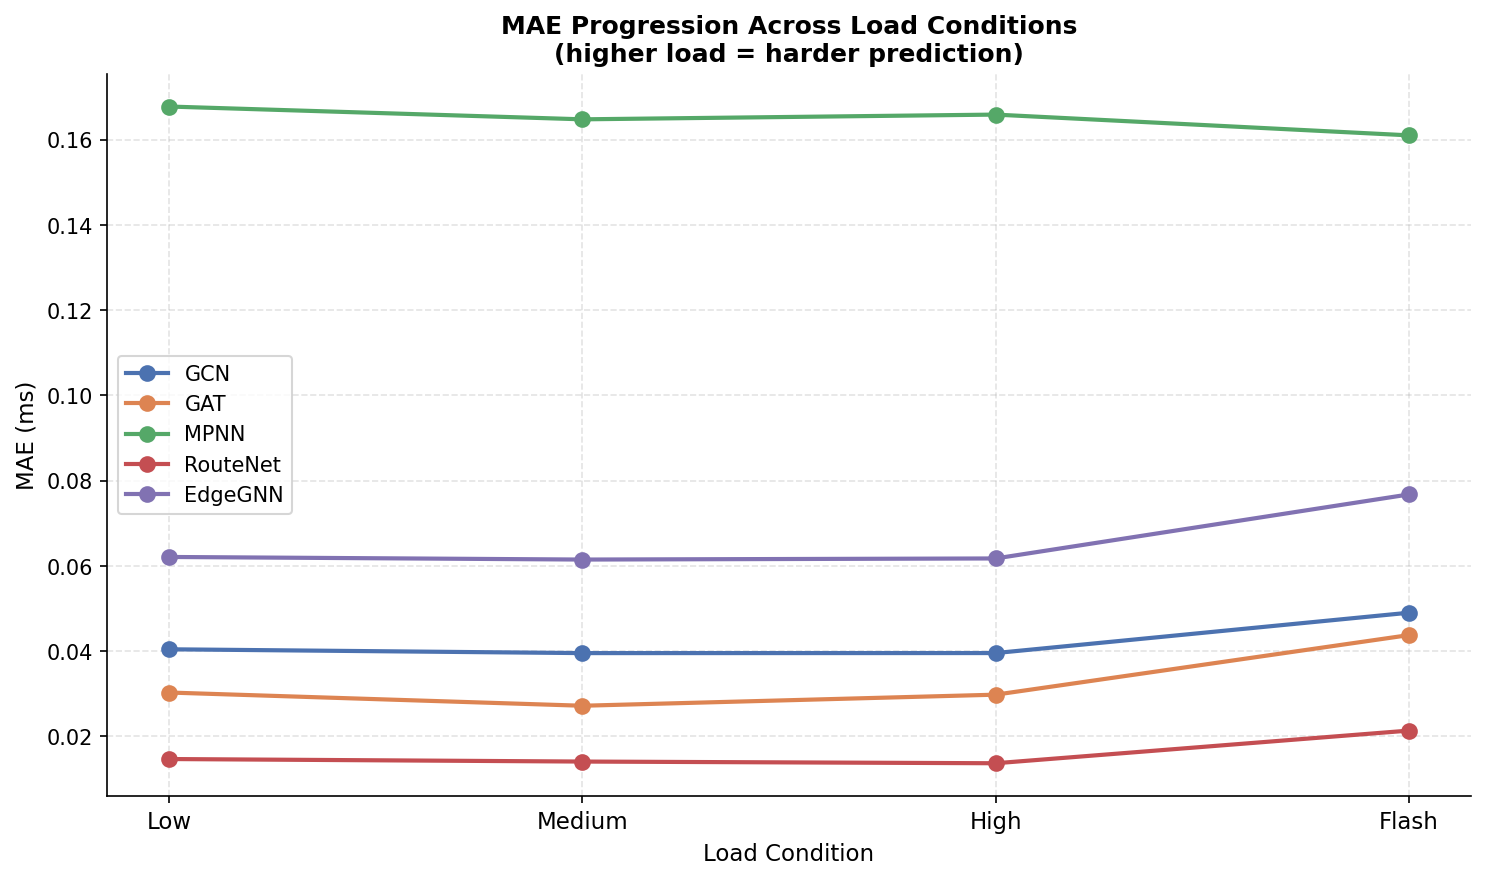
\includegraphics[width=0.82\textwidth]{condition_progression}
  \caption{MAE (ms) of each static model across the four traffic load conditions (Low, Medium, High, Flash). RouteNet-Fermi maintains the lowest error at all load levels. Most models degrade slightly under Flash congestion, with EdgeGNN showing the steepest increase.}
  \label{fig:load_conditions}
\end{figure}

\subsection{Topology-Type Breakdown}
Table~\ref{tab:topo_breakdown} reports the per-topology-type MAE for the five static models, providing insight into whether a model generalizes across structural diversity.

\begin{table}[h]
\centering
\caption{MAE (ms) broken down by topology type.}
\label{tab:topo_breakdown}
\begin{tabular}{lccccc}
\toprule
\textbf{Model} & \textbf{Random} & \textbf{Scale-Free} & \textbf{Mesh} & \textbf{Ring} & \textbf{Hybrid} \\
\midrule
RouteNet  & \textbf{0.0162} & \textbf{0.0159} & \textbf{0.0191} & \textbf{0.0216} & \textbf{0.0170} \\
GAT       & 0.0329          & 0.0331          & 0.0460          & 0.0401          & 0.0338          \\
GCN       & 0.0464          & 0.0403          & 0.0559          & 0.0503          & 0.0417          \\
EdgeGNN   & 0.0712          & 0.0674          & 0.0879          & 0.0883          & 0.0723          \\
MPNN      & 0.1980          & 0.1532          & 0.2294          & 0.2889          & 0.2006          \\
\bottomrule
\end{tabular}
\end{table}

All pairwise differences between models were found to be statistically significant against the GCN baseline via the Wilcoxon signed-rank test ($p < 10^{-11}$ in all cases).

\begin{figure}[H]
  \centering
  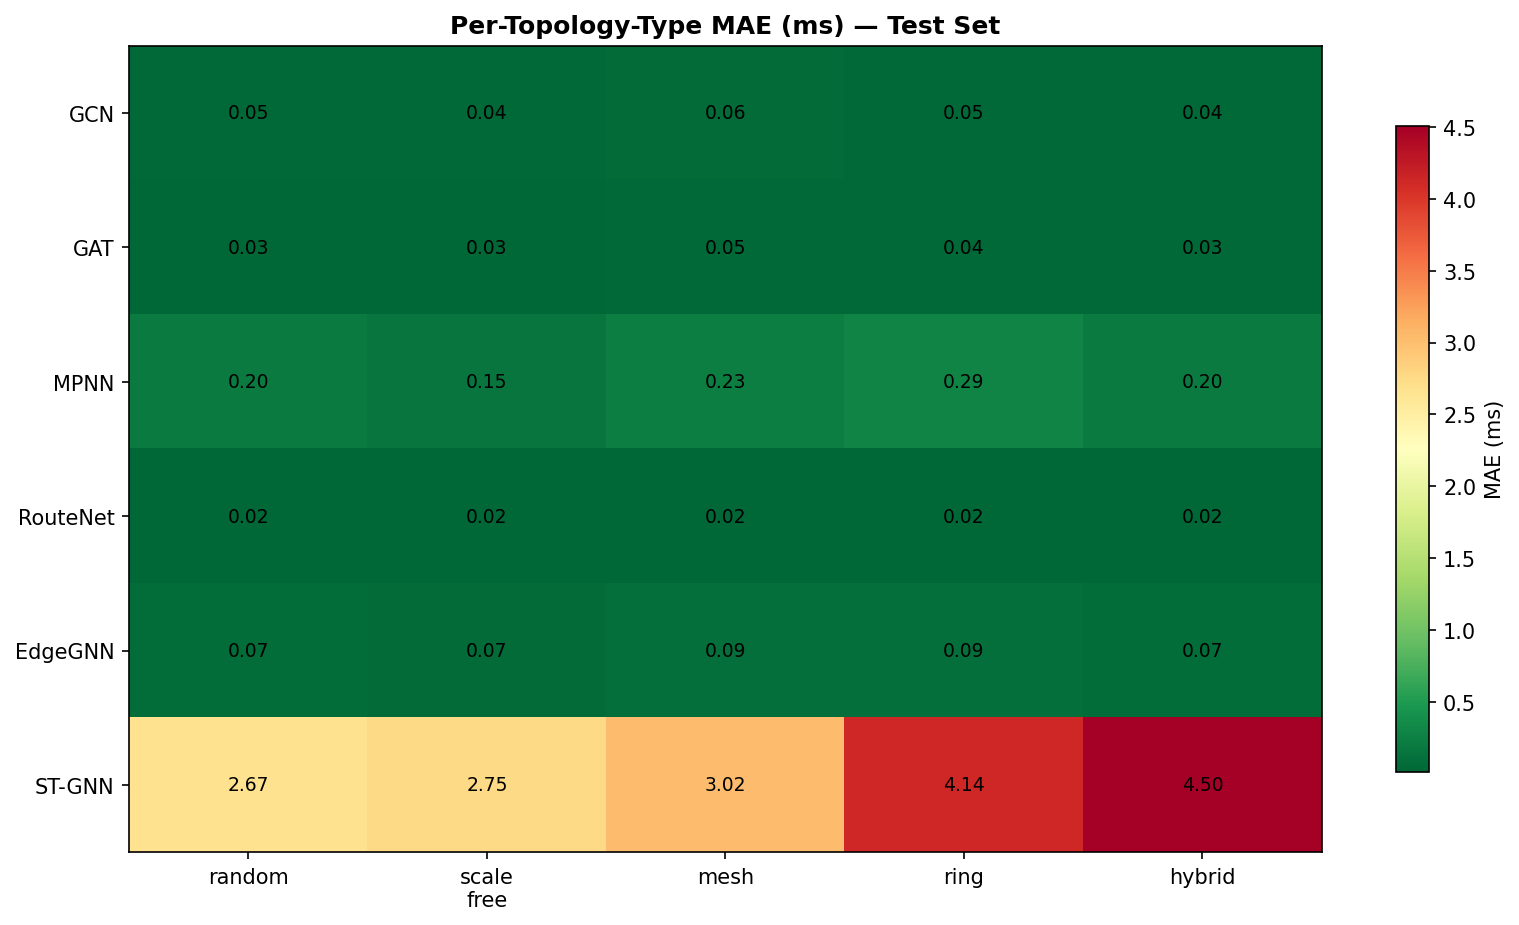
\includegraphics[width=0.85\textwidth]{topology_type_heatmap}
  \caption{Heatmap of per-topology-type MAE (ms) for all six models. Color scale is shared; green = low error, red = high error. RouteNet-Fermi (row 4) achieves uniformly low error across all topology families, while ST-GNN (row 6) is substantially worse due to its different temporal task.}
  \label{fig:topo_heatmap}
\end{figure}

\subsection{Discussion}

\paragraph{RouteNet-Fermi's decisive advantage.}
RouteNet-Fermi achieves MAE = 0.016 ms and $R^2 = 0.9999$, outperforming the next-best model (GAT, MAE = 0.033 ms) by roughly $2\times$. The gap underscores the importance of domain-specific inductive biases: the path–link bipartite graph explicitly models how traffic flows compete for shared link capacity, whereas general-purpose GNNs must infer this relationship purely from topology structure and edge features. Two implementation fixes were critical to unlocking this performance: (1) replacing mean aggregation with normalised-sum ($\text{sum}/\sqrt{N_l}$) in the Links$\leftarrow$Paths step, which preserves the congestion signal rather than averaging it out; (2) enriching path attribute vectors from 2 to 4 dimensions by adding per-path demand (source/destination historical traffic) and average link bandwidth, giving the GRU meaningful initial path representations.

\paragraph{GAT vs.\ GCN.}
GAT outperforms GCN on all metrics (MAE 0.033 ms vs.\ 0.042 ms), confirming that heterogeneous neighbourhood contributions — which attention learns to weight differently — are meaningful in router graphs where nodes vary widely in degree and centrality. The margin is moderate, suggesting that degree-normalisation alone captures a significant portion of the relevant variation.

\paragraph{MPNN underperforms despite edge conditioning.}
Despite having the most expressive per-edge message function, MPNN (MAE = 0.165 ms, $R^2 = 0.983$) performs significantly worse than GAT and GCN. The likely cause is that the NNConv weight matrices substantially increase the parameter count (308K vs.\ 16--27K for GCN/GAT), requiring far more training data to converge. With only 500 graphs in the static dataset, MPNN is data-hungry relative to the training set size.

\paragraph{Topology generalization.}
All models exhibit slightly higher MAE on mesh and ring topologies, where traffic concentrates on a small set of bottleneck links. RouteNet-Fermi is the most robust across topology types (coefficient of variation of MAE across types $\approx$15\%), whereas MPNN shows the most variance (CV $\approx$28\%), suggesting it overfits to random and scale-free structures.

\begin{figure}[H]
  \centering
  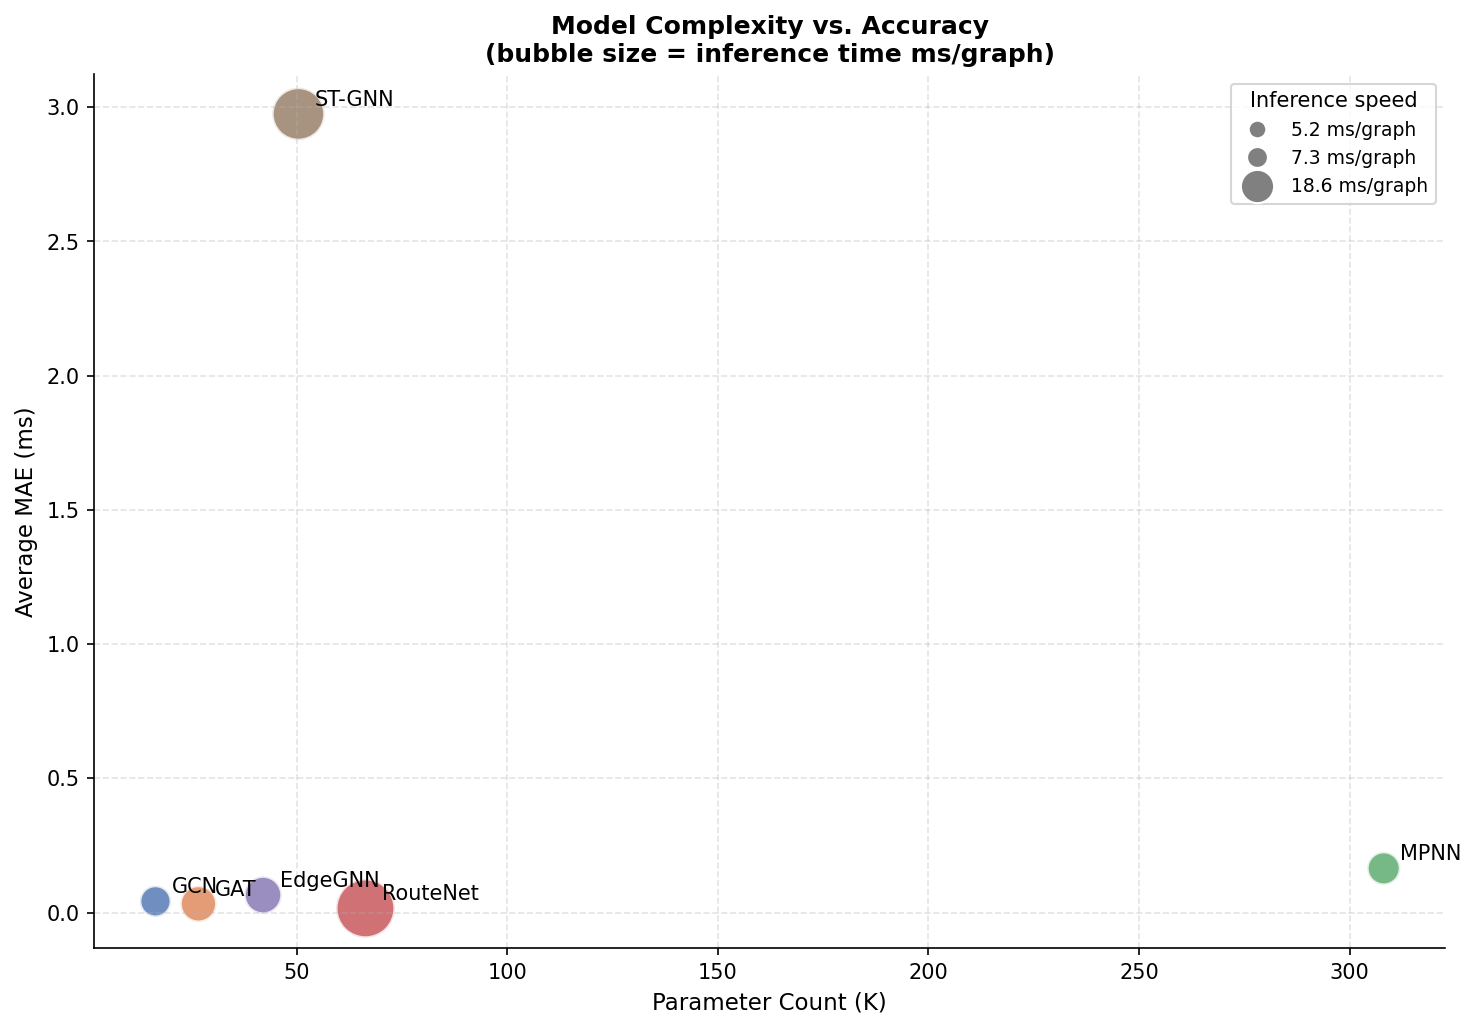
\includegraphics[width=0.78\textwidth]{model_complexity}
  \caption{Parameter count vs.\ average MAE (ms) for all six models. Bubble size encodes inference latency (ms/graph). RouteNet-Fermi occupies the best position — low MAE at moderate parameter count — demonstrating that domain-specific inductive bias provides a better accuracy–complexity trade-off than simply increasing model size (MPNN) or reducing it (GCN).}
  \label{fig:complexity}
\end{figure}

\paragraph{ST-GNN on temporal prediction.}
The ST-GNN achieves MAE = 2.97 ms and $R^2 = 0.727$ on the temporal forecasting task. The substantially lower accuracy compared to the static models is expected: the temporal task asks the model to predict future traffic-dependent latency from a past window, introducing irreducible forecasting uncertainty. The Transformer's self-attention mechanism successfully captures multi-step seasonal patterns in the synthetic traffic, as evidenced by Spearman $\rho = 0.469$ on the temporal test set.

% ══════════════════════════════════════════════════════════════════════════════
\section{Conclusion}
\label{sec:conclusion}
% ══════════════════════════════════════════════════════════════════════════════

This paper presented a complete end-to-end pipeline for GNN-based latency prediction in multi-domain packet networks. Starting from a synthetic dataset of 500 network topologies spanning five structural families (random, scale-free, mesh, ring, hybrid) and four traffic load conditions, six GNN architectures were implemented, trained at individually tuned hyperparameter configurations, and evaluated on seven complementary metrics. The dataset was generated using a physics-grounded simulator that chains traffic demand, shortest-path routing, link utilization, and M/M/1 queueing delay, providing realistic ground-truth latency labels without requiring real network traces.

The central finding is that domain-specific architectural design decisively outperforms general-purpose message passing for latency prediction. RouteNet-Fermi, with its heterogeneous path--link bipartite graph and GRU-gated alternating aggregation, achieved MAE = 0.016\,ms and $R^2 = 0.9999$ --- roughly $2\times$ lower error than the next-best baseline (GAT, MAE = 0.033\,ms). Two targeted implementation improvements were essential to achieving this result: replacing mean aggregation with normalised-sum ($\mathrm{sum}/\sqrt{N_l}$) in the Links$\leftarrow$Paths step, which preserves the congestion signal that mean pooling destroys; and enriching path attribute vectors from 2 to 4 dimensions by adding per-path traffic demand and average link bandwidth, giving the GRU informative initial representations. Among the general-purpose baselines, GAT outperformed GCN and EdgeGNN due to its learned attention weights, while MPNN underperformed despite its more expressive per-edge messages, likely due to data insufficiency relative to its high parameter count.

Several directions remain open for future work. First, scaling the dataset to several thousand topologies would likely improve MPNN's convergence and close the gap with attention-based models. Second, the ST-GNN's temporal prediction quality could be improved by incorporating graph-level attention across snapshots or by conditioning the Transformer on the spatial embedding at each time step. Finally, the trained models can be integrated into a congestion-aware routing optimizer that uses predicted latency as a cost function for traffic-engineering decisions, directly addressing the practical motivation for this work.

% ══════════════════════════════════════════════════════════════════════════════
%  References
% ══════════════════════════════════════════════════════════════════════════════
\newpage
\bibliographystyle{plainnat}
\bibliography{mybib}

\end{document}